\chapter{Between Genes and Traits Lies All of Life}

\begin{kaichang}
Search an online shopping site for genetic testing and find a business offering this: mail saliva, receive a lengthy report on ancestry, alcohol flushing, caffeine metabolism, explosive versus endurance athletic ability, and future disease risks. The advertisements are emphatic: genes hold the answers.

Before ordering, consider a thought experiment. Suppose the report is completely honest and technically reliable, reading your DNA without a single error. Where is the boundary between what it can and cannot tell you? Can it predict the person you will become?

Guess first. By the end, you will have tools to assess every sentence, and discover that misleading reports often owe less to measurement errors than to the language of ``genes are destiny.''
\end{kaichang}

\section{Traits: Settings and Dials}

At the phenomenon level, ignore genes and observe people.

Some traits have a few discrete \textbf{settings}: ABO blood groups are A, B, AB, or O, never ``half-A.'' Reactions to broad beans in favism, and dry versus wet earwax, also largely occupy discrete categories. Others are \textbf{continuous} dials: almost every height from 1.4 to two meters occurs, skin color forms an unbroken spectrum, and blood pressure, weight, and running performance behave similarly.

Identical twins offer a subtler observation. They arise from one fertilized egg and have nearly identical DNA. They certainly resemble each other, often hard to distinguish side by side. Yet acquaintances know their differing personalities, hairstyles, and even fingerprints. If one studies piano and another soccer, their physiques may differ visibly ten years later. Identical sequences do not produce identical finished objects.

Time adds another dimension. Your great-grandparents' generation averaged shorter than people of the same age today, not because genes changed over one century---gene frequencies do not change that fast---but because nutrition, medicine, and childhood illness changed. The same blueprint under different construction conditions produces different building heights.

These three observations---discrete and continuous traits, twin differences, and generational height change---are what we must explain. The key lies in the surprisingly long chain from DNA to trait.

\section{How One Letter Becomes a Disease}

Zoom to particles. To expose every link, follow one well-understood hereditary disease, sickle-cell anemia, as our guide.

Begin in blood. Red cells lack nuclei and are packed with hemoglobin (Chapter 48). Each hemoglobin molecule has four chains, including two $\beta$-globin chains. Their recipe resides in DNA; transcription (Chapter 68) and translation (69) let ribosomes assemble amino acids by codon. Position six normally contains glutamate, whose negatively charged, hydrophilic side chain sits quietly on the protein surface.

In some people's DNA, the corresponding base changes from A to T: Chapter 72's substitution, one among three billion letters. Just one. The codon changes from GAG to GUG, and translation inserts valine instead of glutamate. Valine's side chain is hydrophobic, water-shy like a tiny oil droplet.

What does an oil spot do on a protein surface? Chapter 48 discussed hydrophobic association: water-shy parts tend to cluster away from water. One valine substitution normally causes little trouble, but when red cells release oxygen and hemoglobin changes shape, the spot becomes exposed. Hemoglobin molecules join oil spot to oil spot, polymerizing into rigid fibers. Growing fibers force soft, disc-shaped red cells into curved sickles.

Now follow cells into tissues. Sickle cells are rigid and fragile: they lodge and accumulate in narrow capillaries, blocking blood. Their roughly 120-day lifespan falls to a dozen or so days, and marrow cannot replace them fast enough. Anemia, tissue oxygen shortage, episodes of severe pain, and eventual spleen, kidney, and other organ damage follow. One base difference amplifies step by step into suffering:

\begin{center}
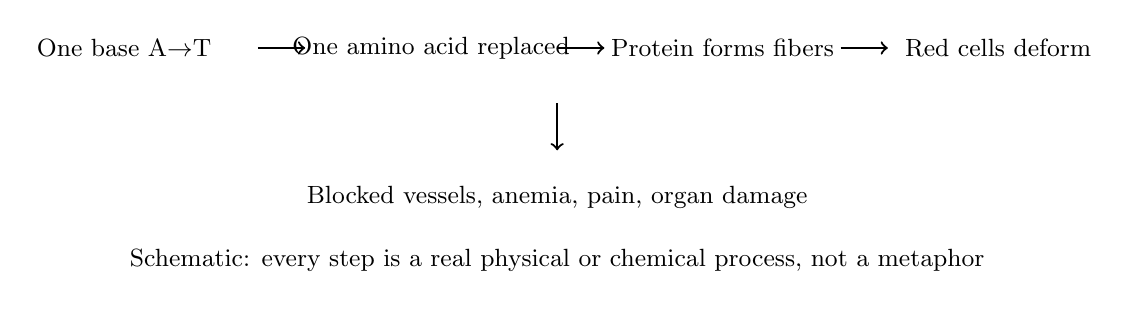
\begin{tikzpicture}[scale=1]
\node[align=center] at (0,0) {\small One base A$\rightarrow$T};
\draw[->, thick] (1.7,0) -- (2.3,0);
\node[align=center] at (3.9,0) {\small One amino acid replaced};
\draw[->, thick] (5.5,0) -- (6.1,0);
\node[align=center] at (7.6,0) {\small Protein forms fibers};
\draw[->, thick] (9.1,0) -- (9.7,0);
\node[align=center] at (11.1,0) {\small Red cells deform};
\draw[->, thick] (5.5,-0.7) -- (5.5,-1.3);
\node[align=center] at (5.5,-1.9) {\small Blocked vessels, anemia, pain, organ damage};
\node[align=center] at (5.5,-2.7) {\small Schematic: every step is a real physical or chemical process, not a metaphor};
\end{tikzpicture}
\end{center}

At every link, information does not act directly; real matter and energy do: hydrophilic and hydrophobic side chains (Chapter 23's water and Chapter 47's lipids), protein shape, cell mechanics, and blood-flow geometry. Genes write only the first line; physics and chemistry perform the rest.

\section{A Network Between Genotype and Phenotype}

With this complete example, state the rule: \textbf{genotype is input and phenotype output, but the intervening network includes proteins, cells, tissues, environment, and history; none can be skipped}.

What does network mean? DNA-to-height requires at least expression levels (Chapter 70), protein folding and modification and partners, cellular division and migration and death (Chapter 75's development), and tissue interactions with hormones, nutrition, and exercise. Other genes and environmental influences enter every level.

Three conceptual pairs follow.

First, \textbf{single-gene versus polygenic}. Traits largely governed by one locus, such as ABO and sickle-cell anemia, are a minority. Quantitative traits like height predominate: genome-wide studies identify hundreds or thousands of associated loci, each contributing millimeters or less, like a vast choir with no soloist. Dozens of genes also regulate melanin type and quantity, so children's skin color often mixes their parents' rather than selecting one of two settings.

Second, \textbf{penetrance and expressivity}. Identical disease genotypes can lead to different outcomes. Penetrance is the fraction of carriers actually showing a trait. Some genotypes have complete penetrance; others do not. Certain pathogenic BRCA1 variants markedly increase breast-cancer risk, yet lifetime occurrence among carriers is roughly sixty to seventy percent, not one hundred. Expressivity describes differing severity among those affected. Homozygous sickle-cell patients may be seriously ill in childhood or have milder symptoms, reflecting other genes, residual fetal hemoglobin, infection history, and medical care. Same genotype and script, different theater and weather.

\textbf{Translator safety note:} The BRCA percentages are source teaching examples, not a personal risk estimate. Consumer tests may miss relevant variants; screening and treatment decisions require clinical interpretation and, where appropriate, genetic counseling. See \href{https://www.cancer.gov/about-cancer/causes-prevention/genetics/brca-fact-sheet}{NCI BRCA guidance}.

Third, \textbf{gene interactions}. A gene's effect often depends on versions of other genes. Tongue rolling, traditionally taught as single-gene inheritance, is actually an excellent counterexample. Identical-twin studies commonly find one roller and one non-roller, and practice can change ability. It is no single-gene yes-or-no test. Genes speak not alone, but through votes around a negotiating table.

Finally, environment is not merely external. Nutrition, childhood infections, sleep, exercise, chronic stress signaling through hormones to the nucleus (Chapter 58), maternal pregnancy nutrition, even developmental order leave traces at every link. Some are remembered without sequence change, by altered use: Chapter 74's epigenetics.

Apply these rules to milk. Nearly all human babies digest lactose using intestinal lactase (Chapter 46). After weaning, most turn lactase expression down (Chapter 70), so adult milk drinking causes bloating and diarrhea: humanity's default. In populations with millennia of dairying, such as northern Europe and East African grasslands, a regulatory variant keeps the light on lifelong, providing valuable calories, calcium, and water. Lactose tolerance reflects a long dance of regulatory variation and dietary culture: sequence supplies hardware, regulation switches, culture environment. Omit any part and you cannot explain why your classmate tolerates milk while you run to the bathroom.

\begin{qiaoliang}
Learn one word correctly: \textbf{heritability}. You have surely seen ``height heritability is $80\%$.'' Most first think, ``Eighty percent of my height is in my genes.'' That is wrong, and correcting it is a central aim here.

Heritability is a \textbf{population statistic}: in a particular population and environment, what fraction of between-person trait \textbf{variation} relates to genetic variation? Eighty percent means genetic differences explain eighty percent of that group's height differences, not eighty percent of your own height. An individual has no such decomposition of between-person variation; you are not a population.

Heritability also changes with environment. Imagine two fields. One has uniform soil and irrigation but varied corn varieties: genetic variety explains almost all height differences, giving nearly $100\%$ heritability. The other uses one variety but fertilizes only half: environment explains almost all variation, giving nearly $0$. The same seeds under a different environmental arrangement yield different heritability. Thus $80\%$ height heritability does not contradict sharply rising average height over a century. Better nutrition and healthcare raise the whole population, while genetic differences still largely explain contemporaneous differences. One statistic, two questions.
\end{qiaoliang}

\section{Compressing the Chain into Symbols}

Now symbols. Chapter 63's allele letters and Punnett squares fit our guide especially well.

Two common $\beta$-globin alleles are normal $\mathrm{Hb^{A}}$ and sickle $\mathrm{Hb^{S}}$. Each person inherits two copies, giving three genotypes and fates:

\begin{table}[h]
\centering
\begin{tabular}{@{}lll@{}}
\toprule
Genotype & Protein level & \shortstack[l]{Individual level\\(phenotype)} \\
\midrule
$\mathrm{Hb^{A}Hb^{A}}$ & All hemoglobin normal & \shortstack[l]{Normal red cells,\\no anemia} \\
$\mathrm{Hb^{A}Hb^{S}}$ & Two hemoglobins mixed & \shortstack[l]{Usually healthy; red cells\\largely retain shape} \\
$\mathrm{Hb^{S}Hb^{S}}$ & Hemoglobin polymerizes & Sickle-cell anemia \\
\bottomrule
\end{tabular}
\end{table}

Symbols compress amazingly: $\mathrm{Hb^{S}}$ holds A-to-T substitution, glutamate-to-valine replacement, and protein polymerization. Compression has a price. ``Usually healthy'' hides expressivity, environment, and gene interactions. Two $\mathrm{Hb^{A}Hb^{S}}$ partners have a $1/4$ probability of an $\mathrm{Hb^{S}Hb^{S}}$ child by Chapter 63's square. That real probability says nothing about severity or quality of life. Symbols give population odds, not personal verdicts.

Estimate how much information gets compressed. Unrelated people's DNA is about $99.9\%$ identical. With roughly $3\times 10^{9}$ bases, two people differ at about
\[3\times 10^{9}\times 0.1\% = 3\times 10^{6}\]
positions, three million. Most lie outside coding and regulatory regions or have no detectable effect. A small subset, playing with the whole environment, differentiates you and your classmate. Remember this when hearing a trait's gene was found: a needle among three million differences, almost never acting alone.

\section{Tracing a Symptom to a Base}

\begin{zhengju}
Nobody deduced the entire base-to-pain chain at a desk. Experiments secured each link over nearly half a century.

The first came under a microscope. In 1910, Chicago physician James Herrick treated a young Caribbean patient with severe anemia and jaundice. A blood smear showed unfamiliar red cells, elongated sickles and crescents rather than discs. He recorded their shapes and named sickle-cell anemia. At that stage he could say only that cell shape was abnormal; genes, DNA, and proteins had not entered.

Thirty-nine years later, the second link arrived. Linus Pauling's 1949 team used electrophoresis, measuring hemoglobin movement in an electric field, which depends on surface charge. Patient and normal hemoglobins moved differently; heterozygous $\mathrm{Hb^{A}Hb^{S}}$ samples contained both. A charge difference changed whole-molecule behavior. Pauling called it the first molecular disease, a revolutionary idea that complex illness could be located in molecular physical properties.

The third link was finer. In 1956, Vernon Ingram fragmented normal and sickle hemoglobin and separated the pieces in two dimensions on paper. Nearly every peptide fingerprint spot matched except one. Analysis revealed a single change among roughly 150 residues: position-six glutamate became valine. One amino acid explained electrophoretic movement; today we know the underlying DNA base change.

The fourth link lay on maps, not in laboratories. High sickle-allele frequencies strikingly overlapped malaria regions in sub-Saharan Africa, the Mediterranean, and parts of India. In 1954, Anthony Allison proposed and tested greater resistance to severe malaria among heterozygotes carrying one $\mathrm{Hb^{S}}$ copy. The overlap was selection's fingerprint, not coincidence. Hold that link for our closing question.

Review the method: morphology asks what is wrong, physics identifies altered molecular charge, chemistry locates an amino acid, and population surveys ask why the variant is common. Every answer generates another question; alternatives such as infection or malnutrition were excluded by controlled experiments. Nobody leapt to the summit, but every link was firmly secured.
\end{zhengju}

\section{Where Does This Model Fail?}

The chain gene $\rightarrow$ protein $\rightarrow$ cell $\rightarrow$ individual is real, but has definite boundaries.

First, \textbf{one gene does not mean one outcome}. Even sickle-cell anemia, a particularly clear hereditary condition with nearly complete penetrance, varies in expressivity. Genotype prediction is reliable; predicting an individual's exact course less so.

Second, \textbf{polygenic traits yield probabilities that can expire}. For height, blood pressure, or diabetes risk, researchers combine small effects at hundreds or thousands of loci into polygenic risk scores. They can help populations, for example prioritizing high-risk groups for screening, but individual errors are striking because effects are small, interactions simplified, and environment important. Worse, most scores use particular ancestry groups and lose accuracy in others. Using them to tell fortunes mistakes population statistics for personal scripts.

Third, \textbf{association is not destiny, probability no deadline}. Triple risk sounds frightening, but a baseline of one in a hundred thousand becomes only three in a hundred thousand. Dose, baseline, and evidence quality, repeatedly emphasized in Volume II, all matter in genetic reports.

\begin{wuqu}
``Height's $80\%$ heritability means genes mostly determine height, so nutrition and intervention do little.'' This swaps population statistics for individual causation. Recall the fields: varieties explain within-field height differences, yet improving water and soil can raise every plant. In reality, average heights rose by over ten centimeters in many countries over a century or two, without time for major gene-pool change. Nutrition, sanitation, and childhood disease changed. Heritability describes why this group differs now, not what everyone would become under a different environment. Using it to dismiss environmental improvement is like treating a thermometer as a radiator's instruction manual.
\end{wuqu}

\begin{shiyan}
\textbf{A Small Family Trait Survey} (safe, using paper and willing relatives).

Materials: paper, pen, and participating relatives, preferably including grandparents.

Steps: List four to six observable traits, such as tongue rolling, attached or free earlobes, backward-bending final thumb joints, preferred hand, and bloating after milk. Ask each relative and record a simple pedigree: squares for males, circles for females, shading for the trait's presence.

Observations: (1) Do any traits show a clear parents-have-it/children-often-have-it pattern? (2) Do identical twins or full siblings ever differ? (3) Which traits seem environmentally influenced, such as handedness altered through education?

Safety: No risk, but an honesty reminder: your observations will reveal that even textbook tongue-rolling inheritance is not supported as a simple allele-pair rule. You need not reach a conclusion; the goal is to encounter the distance from genes to traits firsthand.
\end{shiyan}

\textbf{Translator safety note:} Participation should be voluntary, without judging ability, health, or parentage. Record existing experiences only: do not ask relatives to drink milk, alcohol, or consume other foods to provoke symptoms. A family survey is not a diagnostic test; discuss medical concerns with a qualified professional, as advised in \href{https://medlineplus.gov/genetics/understanding/inheritance/riskassessment/}{MedlinePlus genetic-risk guidance}.

\section{Rereading the Genetic Report}

Return to the saliva sample. You can now assess the report sentence by sentence.

An estimate of East Asian ancestry is a statistical comparison with reference populations, reliable but changeable as databases update, not a bloodline certificate carved in stone.

Prediction of alcohol flushing often reflects a real aldehyde-dehydrogenase variant, one base changing one amino acid, analogous to our sickle-cell chain. Short chain, large effect, high penetrance: this is where genetic reports predict strongly.

\textbf{Translator safety note:} A flushing prediction does not establish a safe amount of alcohol or justify drinking to check it. Flushing can indicate intolerance and elevated cancer risk; see \href{https://www.niaaa.nih.gov/publications/alcohol-flush-reaction-does-drinking-alcohol-make-your-face-red}{NIAAA guidance}.

A claim that you are an explosive-power athlete warrants caution. Athletic ability combines hundreds of genes, training, nutrition, injury history, and psychology. One locus contributes little. An honest version would say a variant has a slight statistical association with certain athletes, too small to guide you individually.

If disease risk is $30\%$ above average, first ask the baseline, then the population used to calculate the score. Remember: risk is population odds, not your script; lifestyle, screening, and medical care can change how it plays out.

A report's value is not spoiling your life story, but handing you cards with different probabilities. Play depends on you and your environment.

\section{Why Have Bad Genes Not Disappeared?}

Leave a question to keep you awake.

Homozygous $\mathrm{Hb^{S}}$ causes serious illness. Intuition says such a bad gene should decline until it vanishes. Yet in many African, Mediterranean, and Indian regions, its frequency reaches $10\%$ or higher. Why?

You know half the answer: overlap with malaria. Heterozygous $\mathrm{Hb^{A}Hb^{S}}$ individuals are not anemic and resist severe malaria, surviving better than either homozygote where malaria is widespread. One allele is both disease and medicine depending on copy number and parasites. Good and bad are not inherent sequence properties, but negotiated with environment.

Who negotiates, under what rules, and why do allele frequencies change across generations? That opens Part X and Chapter 76, natural selection. We return soon.

\begin{tiaozhan}
Compress our intuition into quantitative genetics. Population phenotype variance $V_P$ can be divided:
\[V_P = V_G + V_E + V_{G\times E}\]
$V_G$ reflects genetic differences, $V_E$ environmental differences, and $V_{G\times E}$ their interaction, for example one variant promoting faster growth under the same nutrition. Broad-sense heritability is $V_G$ as a fraction of $V_P$. Three lessons follow. First, heritability is a \textbf{ratio}, with population and environment in both numerator and denominator, so changing either changes it. Second, interactions sometimes prevent separate genetic and environmental accounts because the books are jointly kept. Third, even zero interaction and heritability equal to one do not make environment powerless, as the fields show. Mathematics does not complicate the conclusion; it secures what you already understand against conceptual sleight of hand. This box is optional.
\end{tiaozhan}

\section*{Try It Yourself}

\begin{sikaoti}
\item Map information from $\mathrm{Hb^{S}}$ through mRNA, protein, red cells, and blood vessels to pain. Label each physical or chemical rule. Which link is most susceptible to environment, such as hydration, infection, or medical care?
\item A friend says, ``My height heritability is $80\%$, so of my 1.75 meters, 1.4 meters belong to genes and the rest to environment.'' Identify two errors and explain using the two fields.
\item $\mathrm{Hb^{S}Hb^{S}}$ penetrance approaches $100\%$, but symptoms vary greatly. Use expressivity and the causal chain to explain different outcomes from the same genotype, identifying at least two varying links.
\item Textbooks long claimed tongue rolling is dominant and controlled by one allele pair. If your survey finds counterexamples, such as two rollers with a non-rolling child, what explanations are possible? Which involve environment, which gene interactions?
\item A polygenic score trained in population A performs worse in B. Explain with the gene--environment--network model. Consider allele frequencies, linkage structure, and environmental distributions.
\item One malaria-endemic region has $10\%$ $\mathrm{Hb^{S}}$, another malaria-free region nearly none. Without researching, predict how frequency changes after malaria eradication over several generations, and why. Chapter 76 supplies the full tools.
\end{sikaoti}
